\chapter{Bittien käsittely}

Tietokone käsittelee tietoa sisäisesti bitteinä
eli numeroina 0 ja 1.
Tässä luvussa tutustumme tarkemmin kokonaisluvun
bittiesitykseen sekä bittioperaatioihin,
jotka muokkaavat luvun bittejä.
Osoittautuu, että näistä operaatioista on
monenlaista hyötyä algoritmien ohjelmoinnissa.
% 
% Tyypillinen tekniikka
% on luvun bittiesityksen rinnastaminen joukon
% osajoukkoon.
% Tällöin joukko-operaatiot voi toteuttaa
% tehokkaasti bittioperaatioina ja
% bittiesitystä voi käyttää esimerkiksi
% dynaamisen ohjelmoinnin tilana.

\section{Luvun bittiesitys}

\index{bittiesitys}

Luvun bittiesitys ilmaisee, mistä 2:n potensseista
luku muodostuu. Esimerkiksi luvun 43 bittiesitys on 101011, koska
$43 = 2^5 + 2^3 + 2^1 + 2^0$
eli oikealta lukien bitit 0, 1, 3 ja 5 ovat ykkösiä
ja kaikki muut bitit ovat nollia.

Tietokoneessa luvun bittiesityksen
bittien määrä on kiinteä ja riippuu käytetystä tietotyypistä.
Esimerkiksi C++:n \texttt{int}-tyyppi on tavallisesti 32-bittinen,
jolloin \texttt{int}-luku tallennetaan 32 bittinä.
Tällöin esimerkiksi luvun 43 bittiesitys \texttt{int}-lukuna on seuraava:
\begin{center}
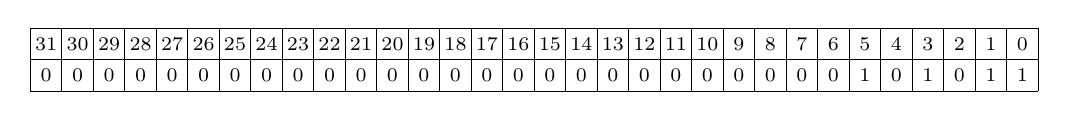
\begin{tikzpicture}[scale=0.4]
\draw (0,0) grid (32,2);
\scriptsize
\node at (31.5,0.5) {1};
\node at (30.5,0.5) {1};
\node at (29.5,0.5) {0};
\node at (28.5,0.5) {1};
\node at (27.5,0.5) {0};
\node at (26.5,0.5) {1};
\foreach \i in {6,...,31}
{
    \node at (31.5-\i,0.5) {0};
}
\foreach \i in {0,...,31}
{
    \node at (31.5-\i,1.5) {\i};
}
\end{tikzpicture}
\end{center}

Luvun bittiesitys on joko etumerkillinen (\textit{signed})
tai etumerkitön (\textit{unsigned}).
Etumerkillisen bittiesityksen ensimmäinen bitti on etumerkki
($+$ tai $-$) ja $n$ bitillä voi esittää luvut $-2^{n-1} \ldots 2^{n-1}-1$.
Jos taas bittiesitys on etumerkitön,
kaikki bitit kuuluvat lukuun ja $n$ bitillä voi esittää luvut $0 \ldots 2^n-1$.

Etumerkillisessä bittiesityksessä ei-negatiivisen luvun
ensimmäinen bitti on 0 ja negatiivisen luvun
ensimmäinen bitti on 1.
Bittiesityksenä on kahden komplementti
(\textit{two's complement}),
jossa positiivisesta luvusta saa negatiivisen muuttamalla
kaikki bitit käänteiseksi ja lisäämällä
tulokseen yksi.

Esimerkiksi luvun $-43$ esitys \texttt{int}-lukuna on seuraava:

\begin{center}
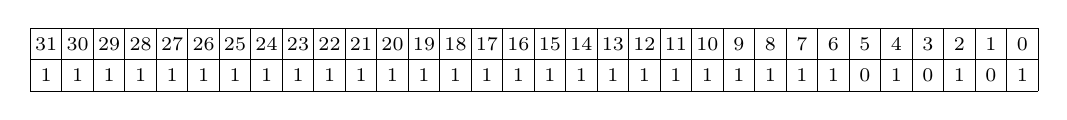
\begin{tikzpicture}[scale=0.4]
\draw (0,0) grid (32,2);
\scriptsize
\node at (31.5,0.5) {1};
\node at (30.5,0.5) {0};
\node at (29.5,0.5) {1};
\node at (28.5,0.5) {0};
\node at (27.5,0.5) {1};
\node at (26.5,0.5) {0};
\foreach \i in {6,...,31}
{
    \node at (31.5-\i,0.5) {1};
}
\foreach \i in {0,...,31}
{
    \node at (31.5-\i,1.5) {\i};
}
\end{tikzpicture}
\end{center}

Etumerkillisen ja etumerkittömän bittiesityksen
yhteys on, että etumerkillisen luvun $-x$
ja etumerkittömän luvun $2^n-x$ bittiesitykset ovat samat.
Niinpä yllä oleva bittiesitys tarkoittaa
etumerkittömänä lukua $2^{32}-43$.

C++:ssa luvut ovat oletuksena etumerkillisiä,
mutta avainsanan \texttt{unsigned} avulla
luvusta saa etumerkittömän.
Esimerkiksi koodissa

\begin{lstlisting}
int x = -43;
unsigned int y = x;
cout << x << "\n"; // -43
cout << y << "\n"; // 4294967253
\end{lstlisting}

etumerkillistä lukua $x=-43$ vastaa etumerkitön luku $y=2^{32}-43$.

Jos luvun suuruus menee käytössä
olevan bittiesityksen ulkopuolelle,
niin luku pyörähtää ympäri.
Etumerkillisessä bittiesityksessä
luvusta $2^{n-1}-1$ seuraava luku on $-2^{n-1}$
ja vastaavasti etumerkittömässä bittiesityksessä
luvusta $2^n-1$ seuraava luku on $0$.
Esimerkiksi koodissa

\begin{lstlisting}
int x = 2147483647
cout << x << "\n"; // 2147483647
x++;
cout << x << "\n"; // -2147483648
\end{lstlisting}

muuttuja $x$ pyörähtää ympäri luvusta $2^{31}-1$ lukuun $-2^{31}$.

\section{Bittioperaatiot}

\newcommand\XOR{\mathbin{\char`\^}}

\subsubsection{And-operaatio}

And-operaatio $x$ \& $y$ tuottaa luvun,
jossa on ykkösbitti niissä kohdissa,
joissa molemmissa luvuissa $x$ ja $y$ on ykkösbitti.
Esimerkiksi $22$ \& $26$ = 18, koska

\begin{center}
\begin{tabular}{rrr}
& 10110 & (22)\\
\& & 11010 & (26) \\
\hline
 = & 10010 & (18) \\
\end{tabular}
\end{center}

And-operaation avulla voi tarkastaa luvun parillisuuden,
koska $x$ \& $1$ = 0, jos luku on parillinen,
ja $x$ \& $1$ = 1, jos luku on pariton.

\subsubsection{Or-operaatio}

Or-operaatio $x$ | $y$ tuottaa luvun,
jossa on ykkösbitti niissä kohdissa,
joissa ainakin toisessa luvuista $x$ ja $y$ on ykkösbitti.
Esimerkiksi $22$ | $26$ = 30, koska

\begin{center}
\begin{tabular}{rrr}
& 10110 & (22)\\
| & 11010 & (26) \\
\hline
 = & 11110 & (30) \\
\end{tabular}
\end{center}

\subsubsection{Xor-operaatio}

Xor-operaatio $x$ $\XOR$ $y$ tuottaa luvun,
jossa on ykkösbitti niissä kohdissa,
joissa tarkalleen toisessa luvuista $x$ ja $y$ on ykkösbitti.
Esimerkiksi $22$ $\XOR$ $26$ = 12, koska

\begin{center}
\begin{tabular}{rrr}
& 10110 & (22)\\
$\XOR$ & 11010 & (26) \\
\hline
 = & 01100 & (12) \\
\end{tabular}
\end{center}

\subsubsection{Not-operaatio}

Not-operaatio \textasciitilde$x$ tuottaa luvun,
jossa kaikki $x$:n bitit on muutettu käänteisiksi.
Operaatiolle pätee kaava \textasciitilde$x = -x-1$,
esimerkiksi \textasciitilde$29 = -30$.

Not-operaation toiminta bittitasolla riippuu siitä,
montako bittiä luvun bittiesityksessä on,
koska operaatio vaikuttaa kaikkiin luvun bitteihin.
Esimerkiksi 32-bittisenä \texttt{int}-lukuna
tilanne on seuraava:

\begin{center}
\begin{tabular}{rrrr}
$x$ & = & 29 &   00000000000000000000000000011101 \\
\textasciitilde$x$ & = & 30 & 11111111111111111111111111100010 \\
\end{tabular}
\end{center}


\subsubsection{Bittisiirrot}

Vasen bittisiirto $x < < k$ tuottaa luvun, jossa luvun $x$ bittejä
on siirretty $k$ askelta vasemmalle
(luvun loppuun tulee $k$ nollabittiä).
Oikea bittisiirto $x > > k$ tuottaa puolestaan
luvun, jossa luvun $x$ bittejä
on siirretty $k$ askelta oikealle 
(luvun lopusta lähtee pois $k$ viimeistä bittiä).

Esimerkiksi $14 < < 2 = 56$,
koska $14$ on bitteinä 1110,
josta tulee bittisiirron jälkeen 111000 eli $56$.
Vastaavasti $49 > > 3 = 6$,
koska $49$ on bitteinä 110001,
josta tulee bittisiirron jälkeen 110 eli $6$.

Huomaa, että vasen bittisiirto $x < < k$
vastaa luvun $x$ kertomista $2^k$:lla
ja oikea bittisiirto $x > > k$
vastaa luvun $x$ jakamista $2^k$:lla
alaspäin pyöristäen.

\subsubsection{Bittien käsittely}

Luvun bitit indeksoidaan oikealta vasemmalle
nollasta alkaen.
Luvussa $1 < < k$ on tarkalleen yksi ykkösbitti
kohdassa $k$, joten sen avulla voi käsitellä
muiden lukujen yksittäisiä bittejä.

Luvun $x$ bitti $k$ on ykkösbitti, jos
$x$ \& $(1 < < k) = (1 < < k)$.
Lauseke $x$ | $(1 < < k)$ asettaa luvun $x$ bitin $k$
ykköseksi, lauseke
$x$ \& \textasciitilde $(1 < < k)$
asettaa luvun $x$ bitin $k$ nollaksi ja
lauseke $x$ $\XOR$ $(1 < < k)$
muuttaa luvun $x$ bitin $k$ käänteiseksi.
% 
% Seuraava koodi muuttaa luvun bittejä:
% 
% \begin{lstlisting}
% int x = 181; // 10110101
% cout << (x|(1<<2)) << "\n"; // 181 = 10110101
% cout << (x|(1<<3)) << "\n"; // 189 = 10111101
% cout << (x&~(1<<2)) << "\n"; // 177 = 10110001
% cout << (x&~(1<<3)) << "\n"; // 181 = 10110101
% cout << (x^(1<<2)) << "\n"; // 177 = 10110001
% cout << (x^(1<<3)) << "\n"; // 189 = 10111101
% \end{lstlisting}
% 
% % Bittiesityksen vasemmanpuoleisin bitti on eniten merkitsevä
% % (\textit{most significant}) ja
% % oikeanpuoleisin bitti on vähiten merkitsevä (\textit{least significant}).

Lauseke $x$ \& $(x-1)$ muuttaa luvun $x$ viimeisen
ykkösbitin nollaksi, ja lauseke $x$ \& $-x$ nollaa
luvun $x$ kaikki bitit paitsi viimeisen ykkösbitin.
Lauseke $x$ | $(x-1)$ vuorostaan muuttaa kaikki
viimeisen ykkösbitin jälkeiset bitit ykkösiksi.

Huomaa myös, että positiivinen luku $x$ on muotoa $2^k$,
jos $x$ \& $(x-1) = 0$.
% 
% Seuraava koodi esittelee operaatioita:
% 
% \begin{lstlisting}
% int x = 168; // 10101000
% cout << (x&(x-1)) << "\n"; // 160 = 10100000
% cout << (x&-x) << "\n"; // 8 = 00001000
% cout << (x|(x-1)) << "\n"; // 175 = 10101111
% \end{lstlisting}

\subsubsection*{Lisäfunktiot}

GCC:n g++-kääntäjä sisältää mm. seuraavat funktiot
bittien käsittelyyn:

\begin{itemize}
\item
$\texttt{\_\_builtin\_clz}(x)$:
nollien määrä bittiesityksen alussa
\item
$\texttt{\_\_builtin\_ctz}(x)$:
nollien määrä bittiesityksen lopussa
\item
$\texttt{\_\_builtin\_popcount}(x)$:
ykkösten määrä bittiesityksessä
\item
$\texttt{\_\_builtin\_parity}(x)$:
ykkösten määrän parillisuus
\end{itemize}

\begin{samepage}
\noindent
Nämä funktiot käsittelevät \texttt{int}-lukuja,
mutta funktioista on myös \texttt{long long} -versiot,
joiden lopussa on pääte \texttt{ll}.

Seuraava koodi esittelee funktioiden käyttöä:

\begin{lstlisting}
int x = 5328; // 00000000000000000001010011010000
cout << __builtin_clz(x) << "\n"; // 19
cout << __builtin_ctz(x) << "\n"; // 4
cout << __builtin_popcount(x) << "\n"; // 5
cout << __builtin_parity(x) << "\n"; // 1
\end{lstlisting}
\end{samepage}

\section{Joukon bittiesitys}

Joukon $\{0,1,2,\ldots,n-1\}$
jokaista osajoukkoa
vastaa $n$-bittinen luku,
jossa ykkösbitit ilmaisevat,
mitkä alkiot ovat mukana osajoukossa.
Esimerkiksi joukkoa $\{1,3,4,8\}$
vastaa bittiesitys 100011010 eli luku
$2^8+2^4+2^3+2^1=282$.

Joukon bittiesitys vie vähän muistia,
koska tieto kunkin alkion kuulumisesta
osajoukkoon vie vain yhden bitin tilaa.
Lisäksi bittimuodossa tallennettua joukkoa
on tehokasta käsitellä bittioperaatioilla.

\subsection{Joukon käsittely}

Seuraavan koodin muuttuja $x$
sisältää joukon $\{0,1,2,\ldots,31\}$
osajoukon.
Koodi lisää luvut 1, 3, 4 ja 8
joukkoon ja tulostaa
joukon sisällön.

\begin{lstlisting}
// x on tyhjä joukko
int x = 0;
// lisätään luvut 1, 3, 4 ja 8 joukkoon
x |= (1<<1);
x |= (1<<3);
x |= (1<<4);
x |= (1<<8);
// tulostetaan joukon sisältö
for (int i = 0; i < 32; i++) {
    if (x&(1<<i)) cout << i << " ";
}
cout << "\n";
\end{lstlisting}
Koodin tulostus on seuraava:
\begin{lstlisting}
1 3 4 8
\end{lstlisting}

\noindent
Nyt joukko-operaatiot voi toteuttaa bittioperaatioilla:
\begin{itemize}
\item $a$ \& $b$ on joukkojen $a$ ja $b$ leikkaus $a \cap b$
(tämä sisältää alkiot,
jotka ovat kummassakin joukossa)
\item $a$ | $b$ on joukkojen $a$ ja $b$ yhdiste $a \cup b$
(tämä sisältää alkiot,
jotka ovat ainakin toisessa joukossa)
\item $a$ \& (\textasciitilde$b$) on joukkojen $a$ ja $b$ erotus
$a \setminus b$ (tämä sisältää alkiot,
jotka ovat joukossa $a$ mutta eivät joukossa $b$)
\end{itemize}

\noindent
Seuraava koodi muodostaa
joukkojen $\{1,3,4,8\}$ ja $\{3,6,8,9\}$ yhdisteen:

\begin{lstlisting}
// joukko {1,3,4,8}
int x = (1<<1)+(1<<3)+(1<<4)+(1<<8);
// joukko {3,6,8,9}
int y = (1<<3)+(1<<6)+(1<<8)+(1<<9);
// joukkojen yhdiste
int z = x|y;
// tulostetaan yhdisteen sisältö
for (int i = 0; i < 32; i++) {
    if (z&(1<<i)) cout << i << " ";
}
cout << "\n";
\end{lstlisting}
Koodin tulostus on seuraava:
\begin{lstlisting}
1 3 4 6 8 9
\end{lstlisting}

\subsection{Osajoukkojen läpikäynti}

Seuraava koodi käy läpi joukon $\{0,1,\ldots,n-1\}$ osajoukot:

\begin{lstlisting}
for (int b = 0; b < (1<<n); b++) {
    // osajoukon käsittely
}
\end{lstlisting}

\noindent
Seuraava koodi käy läpi
osajoukot, joissa on $k$ alkiota:

\begin{lstlisting}
for (int b = 0; b < (1<<n); b++) {
    if (__builtin_popcount(b) == k) {
        // osajoukon käsittely
    }
}
\end{lstlisting}

\noindent
Seuraava koodi käy läpi bittiesitystä
$x$ vastaavan joukon osajoukot:
\begin{lstlisting}
int b = 0;
do {
    // osajoukon käsittely
} while (b=b-x&x);
\end{lstlisting}

Yllä olevien koodien tavoin tämä koodi käy osajoukot
läpi bittiesityksen suuruusjärjestyksessä.

\section{Dynaaminen ohjelmointi}

\subsection{Permutaatioista osajoukoiksi}

Dynaamisen ohjelmoinnin avulla on usein mahdollista
muuttaa permutaatioiden läpikäynti osajoukkojen läpikäynniksi.
Tällöin dynaamisen ohjelmoinnin tilana on
joukon osajoukko sekä mahdollisesti muuta tietoa.

Tekniikan hyötynä on,
että $n$-alkioisen joukon permutaatioiden määrä ($n!$)
on selvästi suurempi kuin osajoukkojen määrä ($2^n$).
Esimerkiksi jos $n=20$, niin $n!=2432902008176640000$,
kun taas $2^n=1048576$.
Niinpä sopivilla $n$:n arvoilla permutaatioita ei ehdi
käydä läpi mutta osajoukot ehtii käydä läpi.

Tutustumme tekniikkaan seuraavan tehtävän kautta:

\begin{task}
Montako permutaatiota voit muodostaa
luvuista $\{ 0,1,\ldots,n-1 \}$ niin,
että missään kohdassa ei ole kahta peräkkäistä lukua?
Esimerkiksi kun $n=4$, ratkaisuja on 2: $(1,3,0,2)$
ja $(2,0,3,1)$.
\end{task}

Merkitään $f(x,k)$:llä,
monellako tavalla osajoukon
$x$ luvut voi järjestää niin,
että viimeinen luku on $k$ ja missään kohdassa
ei ole kahta peräkkäistä lukua.
Esimerkiksi $f(\{0,1,3\},1)=1$,
koska voidaan muodostaa permutaatio $(0,3,1)$,
ja $f(\{0,1,3\},3)=0$, koska 0 ja 1 eivät
voi olla peräkkäin alussa.

Funktion $f$ avulla ratkaisu tehtävään
on summa

\[ \sum_{i=0}^{n-1} f(\{0,1,\ldots,n-1\},i). \]

\noindent
Dynaamisen ohjelmoinnin tilat voi
tallentaa seuraavasti:

\begin{lstlisting}
long long d[1<<n][n];
\end{lstlisting}

\noindent
Perustapauksena $f(\{k\},k)=1$ kaikilla $k$:n arvoilla:

\begin{lstlisting}
for (int i = 0; i < n; i++) d[1<<i][i] = 1;
\end{lstlisting}

\noindent
Tämän jälkeen muut funktion arvot
saa laskettua seuraavasti:

\begin{lstlisting}
for (int b = 0; b < (1<<n); b++) {
    for (int i = 0; i < n; i++) {
        for (int j = 0; j < n; j++) {
            if (abs(i-j) > 1 && (b&(1<<i)) && (b&(1<<j))) {
                d[b][i] += d[b^(1<<i)][j];
            }
        }
    }
}
\end{lstlisting}

\noindent
Muuttujassa $b$ on osajoukon bittiesitys,
ja osajoukon luvuista muodostettu
permutaatio on muotoa $(\ldots,j,i)$.
Vaatimukset ovat, että lukujen $i$ ja $j$
etäisyyden tulee olla yli 1
ja lukujen tulee olla osajoukossa $b$.

Lopuksi ratkaisujen määrän saa laskettua näin
muuttujaan $s$:

\begin{lstlisting}
long long s = 0;
for (int i = 0; i < n; i++) {
    s += d[(1<<n)-1][i];
}
\end{lstlisting}

\subsection{Osajoukkojen määrät}

Dynaamisen ohjelmoinnin avulla voi ratkaista
myös seuraavan tehtävän:

\begin{task}
Tarkastellaan $n$-alkioisen joukon osajoukkoja.
Jokaista osajoukkoa $x$ vastaa arvo $c(x)$.
Tehtäväsi on jokaiselle osajoukolle $x$
summa
\[s(x)=\sum_{y \subset x} c(y) \]
eli bittimuodossa ilmaistuna
\[s(x)=\sum_{y \& x = y} c(y). \]
\end{task}

\noindent
Seuraavassa on esimerkki funktioiden arvoista,
kun $n=3$:

\begin{center}
\begin{tabular}{rrr}
$x$ & $c(x)$ & $s(x)$ \\
\hline
000 & 2 & 2 \\
001 & 0 & 2 \\
010 & 1 & 3 \\
011 & 3 & 6 \\
100 & 0 & 2 \\
101 & 4 & 6 \\
110 & 2 & 5 \\
111 & 0 & 12 \\
\end{tabular}
\end{center}

Esimerkiksi $s(110)=c(000)+c(010)+c(100)+c(110)=7$. 

Tehtävä on mahdollista ratkaista ajassa $O(2^n n)$
laskemalla arvoja funktiolle $f(x,k)$:
mikä on lukujen $c(y)$ summa, missä $y$:n saa $x$:stä
muuttamalla halutulla tavalla bittien $0,1,\ldots,k$
joukossa ykkösbittejä nollabiteiksi.
Tämän funktion avulla ilmaistuna $s(x)=f(x,n-1)$.

Funktion $f$ voi laskea rekursiivisesti seuraavasti:

\begin{equation*}
    f(x,k) = \begin{cases}
               c(x)          & \textrm{jos $k=-1$}\\
               f(x,k-1)          & \textrm{jos $x$:n bitti $k$ on 0}\\
               f(x,k-1)+f(x \XOR (1 < < k),k-1)    & \textrm{jos $x$:n bitti $k$ on 1}\\
           \end{cases}
\end{equation*}

Pohjatapauksena $f(x,-1)=c(x)$,
koska mitään bittejä ei saa muokata.
Muuten jos kohdan $k$ bitti on nolla,
se säilyy nollana, ja jos kohdan $k$ bitti on ykkönen,
se joko säilyy ykkösenä tai muuttuu nollaksi.

Seuraava koodi laskee kaikki funktion $s$ arvot taulukkoon
\texttt{s} olettaen, että funktion $c$ arvot ovat
taulukossa \texttt{c}.
\begin{lstlisting}
for (int b = 0; b < (1<<n); b++) s[b] = c[b];
for (int k = 0; k < n; k++) {
    for (int b = 0; b < (1<<n); b++) {
        if (b&(1<<k)) s[b] += s[b^(1<<k)];
    }
}
\end{lstlisting}
Koodi laskee ensin kaikki arvot funktiolle $f(x,0)$,
sitten kaikki arvot funktiolle $f(x,1)$, jne.